\documentclass[11pt]{report}

\usepackage{geometry} % See geometry.pdf to learn the layout options. There are lots.
\geometry{a4paper} %or letterpaper or a5paper or ... 

%for figures and graphics
\usepackage{graphicx}
\DeclareGraphicsRule{.tif}{png}{.png}{`convert #1 `dirname #1`/`basename #1 .tif`.png}

%\input imports all commands from the target files
%The idea behind this file is that it will be used to store all the maths-related macros that I concoct; so that I can import all the commands by \input{this file} in the preamble of any file that I want to use them in.
%This should make the top-level files look a lot cleaner, and the preamble much shorter!

\usepackage{amssymb}
\usepackage{amsmath}

%theorems and lemma etc setup using amsthm
\usepackage{amsthm}
\newcommand{\tstk}[1]{\textbf{#1} \newline}
\theoremstyle{definition}
\newtheorem{definition}{Definition}[section]
\theoremstyle{plain}
\newtheorem{theorem}{Theorem}[section]
\theoremstyle{plain}
\newtheorem{lemma}[theorem]{Lemma}
\theoremstyle{plain}
\newtheorem{prop}[theorem]{Proposition}

\allowdisplaybreaks %allows equations in the same align environment to split over multiple pages.

%begin the macros via newcommand. Try to group them up reasonably!

%standard sets
\newcommand{\naturals}{\mathbb{N}}			%natural numbers
\newcommand{\integers}{\mathbb{Z}}			%integers
\newcommand{\rationals}{\mathbb{Q}}			%rational numbers
\newcommand{\reals}{\mathbb{R}}				%real numbers
\newcommand{\complex}{\mathbb{C}}			%complex numbers

%brackets and norms
\newcommand{\bracs}[1]{\left( #1 \right)}				%encloses input in brackets
\newcommand{\sqbracs}[1]{\left[ #1 \right]}				%encloses input in square brackets
\newcommand{\clbracs}[1]{\left\{ #1 \right\}}			%encloses input in curly bracers
\newcommand{\abs}[1]{\lvert #1 \rvert}					%absolute value
\newcommand{\norm}[2]{\lvert\lvert #1 \rvert\rvert}		%norm (double line)

%function sets
\newcommand{\smooth}[1]{C^{\infty}\bracs{#1}}							%smooth functions
\newcommand{\ltwo}[2]{L^{2}\bracs{#1,\mathrm{d}#2}}						%general L^2 space
\newcommand{\gradSob}[2]{H^1_\mathrm{grad}\bracs{#1, \mathrm{d}#2}}		%gradient Sobolev space
\newcommand{\curlSob}[2]{H^1_\mathrm{curl}\bracs{#1, \mathrm{d}#2}}		%curl Sobolev space
\newcommand{\kSob}[2]{H^1_{k,\mathrm{curl}}\bracs{#1, \mathrm{d}#2}}	%k-curl Sobolev space

%grad and curl sets
\newcommand{\gradZero}[2]{\mathcal{G}_{ #1, \mathrm{d}#2}\bracs{0}}		%gradients of zero for domain #1 with measure #2
\newcommand{\curlZero}[2]{\mathcal{C}_{ #1, \mathrm{d}#2}\bracs{0}}	%curls of zero for domain #1 with measure #2

%derivatives and grad-like symbols
\newcommand{\diff}[2]{\dfrac{\mathrm{d}#1}{\mathrm{d}#2}}			%complete derivative d#1/d#2
\newcommand{\pdiff}[2]{\dfrac{\partial #1}{\partial #2}}			%partial derivative p#1/p#2
\newcommand{\ddiff}[2]{\dfrac{\mathrm{d}^2 #1}{\mathrm{d}^2 #2}}	%2nd deriv
\newcommand{\grad}{\nabla}											%grad operator
\newcommand{\curl}[1]{\grad_{#1}\wedge}								%curl with measure subscript #1

%displaying integrals
\newcommand{\integral}[3]{\int_{#1}#2 \ \mathrm{d}#3}			%integral, domain #1, integrand #2, measure #3

%notation for variable use throughout the file
\newcommand{\dddom}{\widetilde{\Omega}}			%3D domain notation
\newcommand{\ddom}{\Omega}						%2D domain notation
\newcommand{\dddmes}{\widetilde{\mu}}			%3D measure
\newcommand{\ddmes}{\mu}						%2D measure

\newcommand{\graph}{\mathbb{G}}					%graph variable %maths commands, variables, and other packages
\usepackage{tikz}

%tikz structures and patterns
\usetikzlibrary{patterns}

%this defines a fill pattern called hexagons
\def\hexagonsize{0.2cm}
\pgfdeclarepatternformonly
  {hexagons}% name
  {\pgfpointorigin}% lower left
  {\pgfpoint{3*\hexagonsize}{0.866025*2*\hexagonsize}}%  upper right
  {\pgfpoint{3*\hexagonsize}{0.866025*2*\hexagonsize}}%  tile size
  {% shape description
   \pgfsetlinewidth{1.2pt}
   \pgftransformshift{\pgfpoint{0mm}{0.866025*\hexagonsize}}
   \pgfpathmoveto{\pgfpoint{0mm}{0mm}}
   \pgfpathlineto{\pgfpoint{0.5*\hexagonsize}{0mm}}
   \pgfpathlineto{\pgfpoint{\hexagonsize}{-0.866025*\hexagonsize}}
   \pgfpathlineto{\pgfpoint{2*\hexagonsize}{-0.866025*\hexagonsize}}
   \pgfpathlineto{\pgfpoint{2.5*\hexagonsize}{0mm}}
   \pgfpathlineto{\pgfpoint{3*\hexagonsize+0.2mm}{0mm}}
   \pgfpathmoveto{\pgfpoint{0.5*\hexagonsize}{0mm}}
   \pgfpathlineto{\pgfpoint{\hexagonsize}{0.866025*\hexagonsize}}
   \pgfpathlineto{\pgfpoint{2*\hexagonsize}{0.866025*\hexagonsize}}
   \pgfpathlineto{\pgfpoint{2.5*\hexagonsize}{0mm}}
   \pgfusepath{stroke}
  } 

\newcommand{\Tube}[6][]%
% [further options], width, iterations, inner color, outer color, path definition
{   \colorlet{InColor}{#4}
    \colorlet{OutColor}{#5}
    \foreach \I in {1,...,#3}
    {   \pgfmathsetlengthmacro{\h}{(\I-1)/#3*#2}
        \pgfmathsetlengthmacro{\r}{sqrt(pow(#2,2)-pow(\h,2))}
        \pgfmathsetmacro{\c}{(\I-0.5)/#3*100}
        \draw[InColor!\c!OutColor, line width=\r, #1] #6;
    } 
} %draws a 3D-tube, see https://tex.stackexchange.com/questions/148379/define-a-path-like-command-in-tikz-to-draw-3d-tubes for details
 %tikz things, including importing tikz itself

%labelling hacks
\newcommand\labelthis{\addtocounter{equation}{1}\tag{\theequation}}

%reminders of things to fill in
%\newcommand{\tstk}[1]{\textbf{#1}\newline}

\title{All Work and Results}  % Declares the document's title.
\author{Will Graham (W.Graham@bath.ac.uk) \cite{graham2018citation}}      % Declares the author's name.
\date{\today}      % commenting out this command produces today's date.

%-------------------------------------------------------------------------
%DOCUMENT STARTS

\begin{document}

%TITLE AND CONTENTS ETC; comment out to save computing time
%\maketitle 					%create title
%\tableofcontents 			%have a contents page
%\newpage 					%begin the actual report on a new page

%REPORT BEGINS

%\input chapters one at a time; the references should all match up and can even cross-reference; however you won't get prompts for references across files when editing.
%NB: Can use \include for speed, but then the directory fills up with useless .aux files.
%To save time, comment out sections that aren't being edited. References may disappear but the file will still compile!

%\chapter{Introduction} \label{ch:1Intro}

\section{Motivation}
Optical fibres are the \textit{de facto} industry standard for large telecommunications systems, thanks to their ability to transmit information quickly and with far less signal loss than other methods (such as metal cables).
The technology has rapidly developed since the first optical fibres were fabricated in the 1970s \cite{knight2003photonic} and optical fibres in use today present a balance between several competing factors to deliver a reliable performance.
Factors such as (optical) loss are inherent, brought about by the materials needed to build the fibres; whilst other factors can be influenced by design (group-velocity dispersion) or the fabrication process (which can lead to imperfections and polarisation effects).
Despite the technological developments of the fibres, the underpinning physical processes remain unchanged --- all improvements to the technology have been incremental and largely centre around the manufacturing process.
The fibre will have a core made of a dielectric (non-conducting) material with a given refractive index and will be surrounded by a cladding; another dielectric material of a lower refractive index.
Typically the difference in refractive indices of the core and cladding is very small \tstk{silica fibres and doping, get some numbers}. 
By choosing a lower refractive index for the cladding material than the core, modes of light\footnote{A mode of light is a mono-frequency solution to the governing equations of electromagnetism in the fibre.} can be confined to the core of an optical fibre via the phenomenon of Total Internal Reflection (TIR) \tstk{reference, cba to explain as it's not important to the report}, allowing guided propagation of light over \tstk{actual distance?} hundreds of kilometres.\newline

Photonic crystal fibres (PCFs) are a departure from the setup of core surrounded by cladding \cite{russell2003photonic}; instead relying on the micro-structure of the photonic crystal to alter the optical properties of the fibre it forms.
This microstructure can cause the crystal to exhibit band-gaps; frequency ranges where there are no propagating modes of light in the crystal, despite the existence of propagating modes at lower (and/or higher) frequencies.
These band-gaps allow for light to be confined to core materials previously thought impossible (like air), or even when the core itself consists of vacuum.
This gives rise to the idea of a ``hollow-core fibre"; a PCF with air (or vacuum) as its core material, guiding light at frequencies determined by the band-gaps of the photonic crystal itself.
For the record, PCFs can also be ``solid core", that is have a more conventional material like silica as the core material, or even have metallic cores \tstk{David's paper he gave us}.
Crucially though, PCFs do not use TIR to guide light but rather exploit the fact that light at particular frequencies is confined to the cores simply because it is unable to propagate in the surrounding crystal, due to the optical properties bestowed on the crystal by its micro-structure.
\tstk{illustrative diagram of fibre differences?}

\section{Background}
In physical applications the 2D cross section is often composed of one or more material inclusions, which can give rise to interesting phenomena in the resulting wave propagation problems (such as band-gap spectra).
These inclusions themselves are often arranged in a periodic structure (where applicable), and the model that one considers for a waveguide will inevitably depend on how one chooses to treat these inclusions.
For our approach we shall define a ``waveguide surface" on which to pose our wave propagation problem, and appropriate boundary conditions at the inclusion interfaces.
Such a problem can be arrived at from appropriate treatment of ``high-contrast" media problems; which reduce a problem on a domain with inclusions to a problem on the inclusions with altered boundary data, representing the information from the original problem.
However in the approach we shall be taking, we will look to formulate our model from a measure-theoretic perspective, which will allow us to retain a level of generality surrounding the geometry we choose to impose on our waveguide. 
In the domains with periodic structure in the $\bracs{x_1,x_2}$-plane, we will often assume this periodic structure to extend infinitely and possess a finite period cell, rather than a periodic pattern extending over a finite region of space.
This is because tools such as the Gelfand transform allow us to reduce a problem on an infinite periodic structure to a family of problems on the period cell which parametrised by the so-called quasi-momentum, which we will elaborate on later.
\tstk{this is more about making sure we have some meaning behind being on the spectrum of operators, so might be better kept for that section}
\tstk{literature review, both David's papers on existing modelling techniques and fibre specs, plus from the analysis side (Zhikov etc).}

\section{Setup} \label{sec:Setup}
We wish to study wave propagation problems on waveguide-like structures in a variety of physical contexts, including \tstk{the aforementioned?}
\begin{itemize}
	\item Electromagnetism (photonic crystal fibres),
	\item Elasticity,
	\item Piezo-elasticity.
\end{itemize}
To this end, we shall consider domains of the form $\dddom = \ddom\times I$ where $I\subset\reals$.
The domain $\dddom$ represents the space the waveguide occupies; $\ddom$ represents the 2-dimensional cross-section of the waveguide in the $\bracs{x_1,x_2}$-plane, which is translation invariant along the axis of the waveguide in the $x_3$ direction.
An illustration of this is provided in figure \ref{fig:IntroStrucDiagram}.
\begin{figure}[h!]
	\centering
	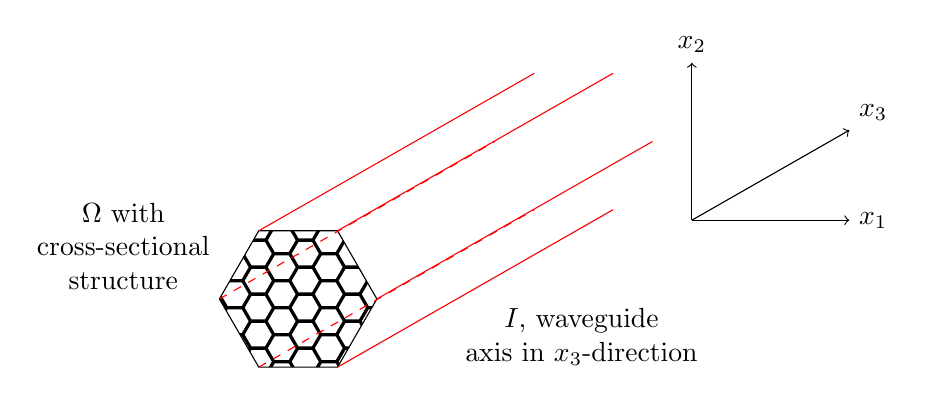
\begin{tikzpicture}
		%2d plane $\ddom$
		\filldraw[pattern=hexagons] (0.5,0.866025) -- (1,0) -- (0.5,-0.866025) -- (-0.5,-0.866025) -- (-1,0) -- (-0.5,0.866025) -- cycle;
		\node[anchor=south east, align=center] at (-1,0) {$\ddom$ with \\ cross-sectional \\ structure};
		
		%1d extension as fibre/waveguide
		\draw[red] (-0.5,0.866025) -- (3, 2.866025);		
		\draw[red] (0.5,0.866025) -- (4, 2.866025);
		\draw[red] (1,0) -- (4.5, 2);
		\draw[red] (0.5,-0.866025) -- (4,2-0.866025);
		\draw[dashed, red] (-0.5,-0.866025) -- (3,2-0.866025);
		\draw[dashed, red] (-1,0) -- (2.5,2);
		\node[anchor=north west, align=center] at (2,0) {$I$, waveguide \\ axis in $x_3$-direction};
		
		%axes labels
		\draw[->] (5,1) -- (7,1) node[anchor=west] {$x_1$};
		\draw[->] (5,1) -- (5,3) node[anchor=south] {$x_2$};
		\draw[->] (5,1) -- (7,1+8/7) node[anchor=south west] {$x_3$};
	\end{tikzpicture}
	\caption{\label{fig:IntroStrucDiagram} Illustration of the waveguide domains that we shall be considering. The domains consist of cross-sectional structure in the $\bracs{x_1,x_2}$-plane which is translation invariant in $x_3$, the direction down the waveguide. The specifics of the structure in the $\bracs{x_1,x_2}$-plane depend on the waveguide we wish to model.}
\end{figure}
The choice of $I$ dictates how we choose to treat the structure we are modelling mathematically; $I=[0,\infty)$ represents a waveguide with an ``entrance" or ``beginning", the choice of $I=\reals$ in the $x_3$-direction represents an ``infinitely long waveguide", and the choice of $I$ being a finite interval represents a waveguide linking two locations. \newline


\chapter{Scalar Equations}
This file should include the work on scalar-gradient equations. This will include construction of the scalar Sobolev spaces, the general theory, and then move into the more specific graph-structure and the edge-equations that we obtain.

\section{Setup}
testing some maths commands...


\section{The Scalar Sobolev Spaces}

\section{An Example System}

%\chapter{Scalar Equations} \label{ch:3VectorEqns}
This file should include the work on vector-curl equations, and have a similar sort of feel to it as the scalar case. Indeed, it should even refer back to the previous section and draw the appropriate parallels.

\section{Setup and Review of Notation}

\section{The Vector Sobolev Spaces}

\section{Curls of Zero - An Example}
This should be the ``everything is a curl of zero" example.

\section{A Waveguide Problem}
The $k$-curls stuff and getting to the edge equations.

\newpage %have a new page to start the bibliography
\bibliographystyle{unsrt}
\bibliography{Bibliography}

\end{document}